% \documentclass[journal=jctcce,manuscript=article]{achemso}
\documentclass[amsmath,amssymb,preprint,aip,jcp]{revtex4-1}
\usepackage[table]{xcolor}
\usepackage{amsmath}
\usepackage{amsfonts}
\usepackage{graphicx}
\usepackage{float}
\usepackage{silence}
\WarningFilter{revtex4-1}{Repair the float}

\begin{document}
\author{Niccol\`{o} Ricardi}
\email{Niccolo.Ricardi@unige.ch}
\author{Cristina E. Gonz\'{a}lez-Espinoza}
\email{Cristina.GonzalezEspinoza@unige.ch}
\author{Tomasz Adam Weso\l{}owski}
\email{Tomasz.Wesolowski@unige.ch}
\affiliation{Department of Physical Chemistry, University of Geneva, Geneva (Switzerland)}
% 
\date{\today}
\title{Negativity of the target density in practical Frozen-Density Embedding Theory based calculations}

\begin{abstract}
The accuracy of any observable derived from multi-scale simulations based on Frozen-Density Embedding Theory (FDET) is affected by two inseparable factors: {\it i}) the approximation for the bi-functional ${E}_{xcT}^{nad}[\rho_A,\rho_B]$ representing the non-additivity of density functionals for the exchange-, correlation-, and kinetic energies and {\it ii}) the possible violation of the non-negativity condition of the target density for a given density associated with the environment $\rho_B(\mathbf{r})$.

The relative significance of theses two factors is investigated for four representative weakly bound intermolecular clusters and various choices for $\rho_B(\mathbf{r})$.
It is shown that the violation of the non-negativity condition of the target density is the principal source of error in the FDET energy
if $\rho_B(\mathbf{r})$ corresponds to the isolated environment.
Reduction of both the magnitude of the violation of the non-negativity condition and the error in the FDET energy can be pragmatically achieved by explicit treatment of the electronic polarisation of the environment.
\end{abstract}

\maketitle

\section{Introduction}\label{sec:intro}
The formal framework of 
Frozen-Density Embedding Theory (FDET) provides the basis of multi-scale/multi-level simulation methods that use a multiplicative embedding operator. The self-consistent expressions for the functional for the total energy and the corresponding functional for embedding potential are available for various possible quantum descriptors of the embedded species \cite{Wesolowski1993,Wesolowski2008,Pernal2009,Wesolowski2015,Wesolowski2020}. 
The environment is described by means of the electron density $\rho_B$ whereas the embedded species by means of the 
embedded $N_A$-electron wavefunction ($\Psi_A$). The total energy of a system is given by the functional ${E}_{v_{AB}}^{FDET}[\Psi_{A},\rho_B]$ which is closely related to the Hohenberg-Kohn energy functional ($E_v^{HK}[\rho]$) known in the density-functional theory \cite{Hohenberg1964} formulation of quantum $N$-electron problem (see Eq.~\ref{eq:nfund} below).

Any multi-level simulation based on the formal framework of FDET
hinges on two types of approximations/assumptions.
One concerns the used approximation for one of the components of ${E}_{v_{AB}}^{FDET}[\Psi_{A},\rho_B]$ the other concerns the approach to generate $\rho_B$. In FDET, multi-level means that $\rho_B$ is generated using other methods than those used to optimise $\Psi_A$. The errors due to these two types of approximations combine and their relative significance cannot be determined in a straightforward matter. The approximation used for ${E}_{v_{AB}}^{FDET}[\Psi_{A},\rho_B]$ leads to errors in the electron density obtained and in errors in energy. The latter can be either positive and negative. The errors due to $\rho_B$ are always non-negative, due to the second Hohenberg-Kohn theorem.
The optimal electron density of the embedded species obtained in FDET, $\rho_A^o$, is always $v$-representable. 
As a result, if $\rho_B$
is larger than the exact ground-state density of the whole system ($\rho_{AB}^o$) on some volume element, the sum of $\rho_A$ and
$\rho_B$ cannot be equal to $\rho_{AB}^o$. Hence, FDET can only provide the upper bound of the exact ground-state anergy of the whole system. The necessary condition to reach the ground-state energy in FDET calculations is the non-negativity of the difference $\rho_{AB}^o-\rho_B$ on all non-zero volume elements.
We will refer to this difference as the {\it target density}.
The condition of non-negativity of $\rho_{AB}^o-\rho_B$ cannot be verified in practice because it requires the {\it a priori} knowledge of 
$\rho_{AB}^o$.

The principal question addressed in the present work is: {\it Does violation of the non-negativity condition matter in practice?} 
The issue has not been studied systematically in the literature.
 There are examples where $\rho_B$ was produced in such a way to not violate the negativity condition. 
Wesolowski and Savin analysed the errors due to approximations used for ${E}_{v_{AB}}^{FDET}[\Psi_{A},\rho_B]$ in a model system for which the exact solutions of FDET are available. Only environment densities such that $\rho_{AB}^o-\rho_B \geq 0$ were considered. \cite{Wesolowski2013}
Fux et al. \cite{Fux2010} used localised Kohn-Sham orbitals from a supermolecular calculation, selecting only those localised on the environment. This led to environment densities whose violation of the non-negativity condition was small and only due to numerical effects. Nonetheless, the authors are not aware of any report of systematic analysis of the effect of sizeable violation extents.

The present work reports the result of a computational experiment on four intermolecular clusters, in which the relative significance 
of the two factors affecting the FDET results is estimated. In such an experiment the density and the energy of the whole cluster $\rho_{AB}^o$ can be evaluated with an adequate method of quantum chemistry and used as a reference for various choices made for $\rho_B$.
In particular, the relation between the violation of the condition of non-negativity of $\rho_{AB}^o-\rho_B$ and the electronic polarisation of the environment due to the interactions with the embedded species is investigated.

The chosen clusters were considered previously in our study of complexation induced shifts in the excitation energies \cite{Ricardi2018} which showed a remarkably good performance of the used FDET-based method despite the fact that the density of the isolated molecule(s) belonging to the environment was used as $\rho_B$ for each electronic excited state. This could be the result of: {\it a}) fortuitous cancellations of errors due to the violation of the non-negativity condition in different electronic states, {\it b}) numerical insignificance of the violation of the non-negativity condition on the total energy, or {\it c}) both. 
For this reason, the present work focusses on one electronic state - the ground-state.
The complexes selected for the present study display different strength of interaction, number of molecules in the environment, number of non-covalent interactions, and the electric charge of the environment:
{\it i}) \textit{cis-}7-hydroxyquinoline bound to two methanol molecules (7HQ-2MeOH), {\it ii}) uracil bound to five water molecules (uracil-5H$_2$O), {\it iii}) 7-hydroxyquinoline bound to formate (7HQ-formate), and {\it iv}) pyridiniumyl benzimidazolide bound to two formic acid molecules (PyrBnz-2HCOOH). 
7HQ-2MeOH and uracil-5H$_2$O are typical hydrogen bonded complexes involving neutral donor and acceptor molecules. 7HQ-formate and PyrBnz-2HCOOH) represent more peculiar cases. In 7HQ-formate, the environment acts as the hydrogen acceptor and is negatively charged. Moreover, the hydrogen is almost shared between the \textit{cis}-7-hydroxyquinoline and the formate: the bond legth of the hydroxy group is 1.09 {\AA} while the hydrogen bond length is 1.36 {\AA}. 
In PyrBnz-2HCOOH, the embedded system (PyrBnz) is a hydrogen acceptor and the atom involved carries a significant negative charge.
\section{Methods}
\subsection{FDET and its extension for non-variational methods}
%\subsubsection{FDET energy functional} 
FDET concerns a system of $N_{AB}$ electrons in an external potential $v_{AB}(\mathbf{r})$.
For interpretation purposes, it is convenient to split the external potential $v_{AB}(\mathbf{r})$ into components $v_{AB}(\mathbf{r})=v_{A}(\mathbf{r})+v_{B}(\mathbf{r})$. 
The embedded wavefunction and the total energy obtained from FDET do not depend on such splitting. 
Once $v_{AB}(\mathbf{r})$ is split, $v_{A}(\mathbf{r})$ defines a $N_A$-electron Hamiltonian ($\hat{H}_A$) whereas 
$v_{B}(\mathbf{r})$ defines a $N_B$-electron Hamiltonian ($\hat{H}_B$). 
The FDET energy functional reads: 
\begin{eqnarray} 
\label{eq:E_FDET_v'}
{E}_{v_A,v_B}^{FDET}[\Psi_{A},\rho_B] = \langle\Psi_{A}\vert \hat{H}_A\vert \Psi_{A}\rangle + E^{HK}_{v_B}[\rho_B] + E^{elst,int}_{v_A,v_B}[\rho_A,\rho_B] + E_{xcT}^{nad}[\rho_A,\rho_B], 
\end{eqnarray}
where {\it i}) $\rho_A(\mathbf{r})=\langle\Psi_A\vert\sum_{i=1}^{N_{A}}\delta(\mathbf{r}_i-\mathbf{r})\vert\Psi_A\rangle$,
{\it ii}) $E^{elst,int}_{v_A,v_B}[\rho_A,\rho_B]$ collects all classical electrostatic contributions to the interaction energy, and 
{\it iii}) $E_{xcT}^{nad}[\rho_A,\rho_B]$ - the definition of this bi-functional depends on the form of the embedded wavefunction\cite{Wesolowski2008}.

The FDET energy functional is defined to satisfy the following relation:
\begin{equation}\label{eq:nfund}
\min_{\Psi_A\rightarrow N_A} E_{v_{A},{v_B}}^{FDET}[\Psi_{A},\rho_B] = E_{v_{A},{v_B}}^{FDET}[\Psi^{o}_{A},\rho_B] = E_{v_{AB}}^{HK}[\rho_A^{o}+\rho_B] \ge E_{v_{AB}}^o,
\end{equation}
where $\rho_A^{{o}}(\mathbf{r})=\langle\Psi_A^{{o}}\vert\sum_{i=1}^{N_{A}}\delta(\mathbf{r}_i-\mathbf{r})\vert\Psi_A^{{o}}\rangle$, $\int\rho_B(\mathbf{r})d\mathbf{r}=N_B$, and $E_{v_{AB}}^o$ is the ground-state energy of the $N_A+N_B$-electron system defined by the potential $v_{A}(\mathbf{r})+v_{B}(\mathbf{r})$.

If the density $\rho^{o}_{AB}-\rho_{B}$ is $v$-representable, $\rho_A^{o}$ defined in Eq.~\ref{eq:nfund} can be obtained from the Euler-Lagrange equation:
\begin{eqnarray}
 \left( \hat{H}_A + \hat{v}_{emb}^{{FDET}}[\rho_A^{{o}}, \rho_B; v_B] \right) \Psi_A^{{o}} &=& \lambda^{o}\Psi_A^{{o}} \label{eq:FDET_SE} 
\end{eqnarray}
where $v_{emb}^{{FDET}}[\rho_A,\rho_B; v_B]$
is the FDET embedding potential:
\begin{eqnarray}
v_{emb}^{{FDET}}[\rho_A,\rho_B; v_B](\mathbf{r}) &=& v_B(\mathbf{r}) + \int \frac{\rho_B(\mathbf{r}')}{|\mathbf{r}-\mathbf{r}'|} d\mathbf{r}'+ \frac{\delta E_{xct}^{nad}[\rho_A,\rho_B]}{\delta\rho_A(\mathbf{r})}.
\label{eq:nFDET_embpot} 
\end{eqnarray}
The term $\frac{\delta E_{xct}^{nad}[\rho_A,\rho_B]}{\delta\rho_A(\mathbf{r})}\equiv v_{xct}^{nad}[\rho_A,\rho_B](\mathbf{r})$ depends on the form of the embedded wavefunction\cite{Wesolowski2008}.
For a single determinant, the FDET expression for $E_{xct}^{nad}[\rho_A,\rho_B]$ includes also the correlation functional $E_c[\rho_A]$ assuring that the optimal embedded density satisfies Eq.~\ref{eq:nfund}. 
In the present work, $E_{xct}^{nad}[\rho_A,\rho_B]$ always denotes the bifunctional corresponding to the embedded wavefunction of the Full Configuration Interaction form\cite{Wesolowski2008}, i.e. $E_c[\rho_A]$ is not included.
The $\rho_A$-dependency of $v_{xct}^{nad}[\rho_A,\rho_B](\mathbf{r})$ leads to two 
particular features of Eq. \ref {eq:FDET_SE}: {\it i}) solving it involves an iterative procedure leading to self-consistency\cite{Dulak2009} and {\it ii}) the Lagrange multiplier $\lambda^{o}$ does not represent the energy.\cite{Zech2016}

We consider the case where the wavefunction $\Psi_A$ in Eq.~\ref{eq:FDET_SE} has a single-determinant form, which we denote with the letter $\Phi$. 
The potential
\begin{eqnarray}
v'_A(\mathbf{r})=v_A(\mathbf{r})+v_{emb}^{{FDET}}[\rho'_A,\rho_B; v_B](\mathbf{r})\label{eq:def_v'},
\end{eqnarray}
where $\rho'_A(\mathbf{r})=\langle\Phi'_A\vert\sum_{i=1}^{N_{A}}\delta(\mathbf{r}_i-\mathbf{r})\vert\Phi'_A\rangle$, defines an auxiliary $N_A$-electron system. The use of a prime ($'$) in the notation ($\Phi'_A$, $\rho'_A$, and $v'_A$) indicates the simultaneous use of a single determinant wavefunction and the neglect of $E_c[\rho_A]$ and its functional derivative. We bring the reader's attention that $\rho'_A$ always denotes the density obtained from a self-consistent single determinant.

According to the recently derived formula relating the quantities available in methods treating the correlation energy of embedded electrons non-variationally to the Hohenberg-Kohn energy functional (Eq. 38 in Ref. \citenum{Wesolowski2020}): 
\begin{eqnarray} \label{eq:E_FDET_gnovc}
 E_{v_{AB}}^{HK}[\rho_A^{o}+\rho_B] &=& E_{v_{A},{v_B}}^{FDET}[\Phi'_{A},\rho_B] + E^{c}_{v'_A} 
 % {E}^{HK}_{v_B}[\rho_B] 
 \\ \nonumber
 &-& E_k[\Delta \rho^{c}_{v'_A}, \rho'_A, \rho_B] + O(\Delta\rho)^2, 
 \end{eqnarray}
%\mathrm{where}&& \nonumber\\
where,
\begin{eqnarray}
\label{eq:nkernel}
 E_k[\Delta \rho^{c}_{v'_A}, \rho'_A, \rho_B] &=&
 \int \rho'_A(\mathbf{r}) \int \Delta \rho^{c}_{v'_A}(\mathbf{r'}) f^{nad}_{xcT}[\rho'_A, \rho_B](\mathbf{r},\mathbf{r'})d\mathbf{r'}\mathrm{d}\mathbf{r},\\
 \nonumber \\ \label{eq:def_corrdens}
 \Delta \rho^{c}_{v'_A}(\mathbf{r})&=&\rho^{o}_{v'_A}(\mathbf{r})-\rho'_{v'_A}(\mathbf{r})\\
 \nonumber \\
 \label{eq:nf_nad}
 f^{nad}_{xcT}[\rho_A, \rho_B](\mathbf{r},\mathbf{r'}) &=& \frac{\delta^2 E^{nad}_{xcT}[\rho_A, \rho_B]}{\delta \rho_A(\mathbf{r}) \delta \rho_A(\mathbf{r'})}.
\end{eqnarray}
$\rho_A^{o}(\mathbf{r})$ in the left-hand side is the optimal correlated density defined in Eq.~\ref{eq:nfund}. 
The right-hand-side of Eq.~\ref{eq:E_FDET_gnovc} is used to approximate $E_{v_{AB}}^{HK}[\rho_A^{o}+\rho_B]$.
Any post-Hartree-Fock method, applied to the potential $v'_A$ (cf. Eq.~\ref{eq:def_v'}), yields the necessary terms: {\it i})
the optimal single determinant ($\Phi'_{A}$), {\it ii}) the corresponding density ($\rho'_{A}$), 
{\it iii}) the correlation energy ($E^{c}_{v'_A}$), and {\it iv}) the change of the density due to correlation ($\Delta \rho^{c}_{v'_A}(\mathbf{r})$). 

For $\Delta\rho$ representing the correlation-induced changes of energy in the exact and in the auxiliary system, 
 $O(\Delta\rho)^2$ collects all second- and higher-order contributions to the energy. 
As far as the $E^{HK}_{v_B}[\rho_B]$ component of ${ E}_{v_A,v_B}^{FDET}[\Psi_{A},\rho_B]$ is concerned,
its treatment depends on the method used to generate $\rho_B$ and will be given below.

For a given $\rho_B(\mathbf{r})$,
the FDET interaction energy is given by:
\begin{eqnarray}
E_{int}^{FDET(\rho_B)}=E_{v_{AB}}^{HK}[\rho_A^{o}+\rho_B] - E_{v_A}^{HK}[\rho_A^{isol}] - 
E_{v_B}^{HK}[\rho_B^{isol}], \label{eq:eint0}
\end{eqnarray}
where $\rho_X^{isol}$ denotes the density of the isolated subsystem $X$.

Using for $E_{v_{AB}}^{HK}[\rho_A^{o}+\rho_B]$ for the right-hand side of Eq.~\ref{eq:E_FDET_gnovc} with neglected $O(\Delta\rho)^2$, results in:
\begin{eqnarray}
E_{int}^{FDET(\rho_B)}&=&
\langle\Phi'_{A}\vert \hat{H}_{v_A}\vert \Phi'_{A}\rangle + E^{c}_{v'_A}
+ E^{elst,int}_{v_A,v_B}[\rho'_A,\rho_B] + {E}_{xcT}^{nad}[\rho'_A,\rho_B] \label{eq:eint1}\\
&-& E_k[\Delta \rho^{c}_{v'_A}, \rho'_A, \rho_B] - E_{v_A}^{HK}[\rho_A^{isol}] + {E}^{HK}_{v_B}[\rho_B] - 
E_{v_B}^{HK}[\rho_B^{isol}] \nonumber
\end{eqnarray}
In the above equation, the quantities: $\Phi'_{A}$, $\rho'_A$, $E^{c}_{v'_A}$, and $\Delta \rho^{c}_{v'_A}$ implicitly depend on $\rho_B$, through $v'_A$. For the sake of conciseness, this dependency is not indicated explicitly. 
\subsection{FDET interaction energy}
The following sub-sections concerns application of Eq.~\ref{eq:eint1} for different choices of $\rho_B$. 
\subsubsection{FDET interaction energy for $\rho_B=\rho_B^{isol}$}
If the environment is modelled by means of its isolated density $\rho_B^{isol}(\mathbf{r})$, the last two terms in Eq.~\ref{eq:eint1} are equal and thus cancel out leading to:
\begin{eqnarray}
E_{int}^{FDET(\rho_B^{isol})}&=&
\langle\Phi'_{A}\vert \hat{H}_{v_A}\vert \Phi'_{A}\rangle + E^{c}_{v'_A}
+ E^{elst,int}_{v_A,v_B}[\rho'_A,\rho_B^{isol}] \label{eq:eint2}\\
&+& {E}_{xcT}^{nad}[\rho'_A,\rho_B^{isol}] - E_k[\Delta \rho^{c}_{v'_A}, \rho'_A, \rho_B^{isol}] - 
\langle\Phi_{A}\vert \hat{H}_{v_A}\vert \Phi_{A}\rangle - E^{c}_{v_A}
%E_{v_A}^{HK}[\rho_A^{isol}] 
\nonumber
\end{eqnarray}
where the exact relation $E_{v_A}^o=E_{v_A}^{HK}[\rho_A^{isol}]=\langle\Phi_{A}\vert \hat{H}_{v_A}\vert \Phi_{A}\rangle + E^{c}_{v_A}$ was used for the energy of the isolated subsystem $A$.
\subsubsection{FDET interaction energy for $\rho_B^{v"}(\mathbf{r})$ being the ground-state Hartree-Fock density for some 
 potential $v"(\mathbf{r})$} 
If the environment density is obtained as Hartree-Fock solution for an external potential $v''(\mathbf{r})$ other than the nuclear potential of subsystem B ($v_B(\mathbf{r})$), the numerical value of 
${E}^{HK}_{v_B}[\rho_B^{v"}]-{E}^{HK}_{v_B}[\rho_B^{isol}]\ge 0$ contributes to the interaction energy. 
It is approximated as:
\begin{eqnarray}
{E}^{HK}_{v_B}[\rho_B^{v"}]=\langle\Phi"_{B}\vert \hat{H}_{v_B}\vert \Phi"_{B}\rangle+E^{c}[\rho_B^{v"}] \approx \langle\Phi"_{B}\vert \hat{H}_{v_B}\vert \Phi"_{B}\rangle+E^{c}_{v"}, \label{eq:evb} 
\end{eqnarray}
where $\Phi"_{B}$ is the optimal determinant yielding $\rho_B^{v"}$ (not the Hartree-Fock wavefunction for $N_B$ electrons in the potential ${v_B}(\mathbf{r})$!).

Using the above approximation in Eq.~\ref{eq:eint1} leads to:
 \begin{eqnarray}
E_{int}^{FDET(\rho_B^{v"})} 
&=& \langle\Phi'_{A}\vert \hat{H}_{v_A}\vert \Phi'_{A}\rangle + E^{c}_{v'_A} + \langle\Phi"_{B}\vert \hat{H}_{v_B}\vert \Phi"_{B}\rangle + E^{c}_{v"} \label{eq:eint3}\\ \nonumber
&+& E^{elst,int}_{v_A,v_B}[\rho'_A,\rho_B^{v"}] + {E}_{xcT}^{nad}[\rho'_A,\rho_B^{v"}]- E_k[\Delta \rho^{c}_{v'_A}, \rho'_A, \rho_B^{v"}] \nonumber\\
&-& 
\langle\Phi_{A}\vert \hat{H}_{v_A}\vert \Phi_{A}\rangle - E^{c}_{v_A}
- \langle\Phi_{B}\vert \hat{H}_{v_B}\vert \Phi_{B}\rangle - E^{c}_{v_B}\nonumber
\end{eqnarray}
where $\Phi_{X}$ is the Hartree-Fock wavefunction and $E^{c}_{v_X}$ denotes the correlation energy in the system defined by the potential $v_X$ ($X=A$ or $B$).
\subsubsection{FDET interaction energy for optimised $\rho_B$}
Optimisation of both $\rho_A$ and $\rho_B$ proceeds by performing an iterative cycle (\textit{freeze-and-thaw}, $FAT$) in which the
subsystem $A$ and $B$ exchange their roles in all FDET equations \cite{Wesolowski1996a}. 
In case of freezing $\rho_A$, $\rho_B$ is represented be means of an embedded $N_B$ electron single determinant ($\Phi'_B$) that is optimal for a given $\rho_A$. Let us denote the quantities obtained at the end of such an optimisation with: $v'^{FAT}_A$, $\Phi'^{FAT}_A$, $\rho'^{FAT}_A$, 
 $E^{c}_{v'^{FAT}_A}$, and $\Delta \rho^{c}_{v'^{FAT}_A}$ for the subsystem $A$ and
 $v'^{FAT}_B$ $\Phi'^{FAT}_B$, $\rho'^{FAT}_B$, 
 $E^{c}_{v'^{FAT}_B}$, and $\Delta \rho^{c}_{v'^{FAT}_A}$ for the subsystem $B$. Using this notation, Eq.~\ref{eq:eint3} reads: 
 \begin{eqnarray}
E_{int}^{FDET(\rho'^{FAT}_B)} 
&=& \langle\Phi'^{FAT}_{A}\vert \hat{H}_{v_A}\vert \Phi'^{FAT}_{A}\rangle + E^{c}_{v'^{FAT}_A} + \langle\Phi'^{FAT}_{B}\vert \hat{H}_{v_B}\vert \Phi'^{FAT}_{B}\rangle + E^{c}_{v'^{FAT}_B} \label{eq:eint4A}\\ \nonumber
&+& E^{elst,int}_{v_A,v_B}[\rho'^{FAT}_A,\rho_B'^{FAT}] + {E}_{xcT}^{nad}[\rho'^{FAT}_A,\rho'^{FAT}_B]- E_k[\Delta \rho^{c}_{v'^{FAT}_A}, \rho'^{FAT}_A, \rho^{FAT}_B] \nonumber\\
&-& 
\langle\Phi_{A}\vert \hat{H}_{v_A}\vert \Phi_{A}\rangle - E^{c}_{v_A}
- \langle\Phi_{B}\vert \hat{H}_{v_B}\vert \Phi_{B}\rangle - E^{c}_{v_B}\nonumber
\end{eqnarray}

If the subsystems A and B exchange their roles in FDET equations (subsequent \textit{freeze-and-thaw} iteration), the corresponding 
expression reads:
 \begin{eqnarray}
E_{int}^{FDET(\rho'^{FAT}_A)} 
&=& \langle\Phi'^{FAT}_{B}\vert \hat{H}_{v_B}\vert \Phi'^{FAT}_{B}\rangle + E^{c}_{v'^{FAT}_B} + \langle\Phi'^{FAT}_{A}\vert \hat{H}_{v_A}\vert \Phi'^{FAT}_{A}\rangle + E^{c}_{v'^{FAT}_A} \label{eq:eint4B}\\ \nonumber
&+& E^{elst,int}_{v_B,v_A}[\rho'^{FAT}_B,\rho_A'^{FAT}] + {E}_{xcT}^{nad}[\rho'^{FAT}_B,\rho'^{FAT}_A]- E_k[\Delta \rho^{c}_{v'^{FAT}_B}, \rho'^{FAT}_B, \rho^{FAT}_A] \nonumber\\
&-& 
\langle\Phi_{B}\vert \hat{H}_{v_B}\vert \Phi_{B}\rangle - E^{c}_{v_B}
- \langle\Phi_{A}\vert \hat{H}_{v_A}\vert \Phi_{A}\rangle - E^{c}_{v_A}\nonumber
\end{eqnarray}
Following Eq.~\ref{eq:E_FDET_gnovc}, both above expressions yield $E_{v_{AB}}^{HK}[\rho'^{FAT}_A+\rho'^{FAT}_B]$ up to the second order terms ($O(\Delta\rho)^2$). 
Adding Eqs.~\ref{eq:eint4A} and \ref{eq:eint4B} and dividing the sum by two yields an expression for the interaction energy that is symmetric upon exchange $A$ and $B$.
\begin{eqnarray}
E_{int}^{FDET(FAT)} 
&=& \langle\Phi'^{FAT}_{B}\vert \hat{H}_{v_B}\vert \Phi'^{FAT}_{B}\rangle + E^{c}_{v'^{FAT}_B} + \langle\Phi'^{FAT}_{A}\vert \hat{H}_{v_A}\vert \Phi'^{FAT}_{A}\rangle + E^{c}_{v'^{FAT}_A} \label{eq:eint4}\\ \nonumber
&+& E^{elst,int}_{v_B,v_A}[\rho'^{FAT}_B,\rho_A'^{FAT}] + {E}_{xcT}^{nad}[\rho'^{FAT}_B,\rho'^{FAT}_A] \nonumber \\
&-& \frac{1}{2}\left(E_k[\Delta \rho^{c}_{v'^{FAT}_A}, \rho'^{FAT}_B, \rho^{FAT}_A] + E_k[\Delta \rho^{c}_{v'^{FAT}_B}, \rho'^{FAT}_A, \rho^{FAT}_B] \right) \nonumber\\
&-& 
\langle\Phi_{B}\vert \hat{H}_{v_B}\vert \Phi_{B}\rangle - E^{c}_{v_B}
- \langle\Phi_{A}\vert \hat{H}_{v_A}\vert \Phi_{A}\rangle - E^{c}_{v_A}\nonumber
\end{eqnarray}
%\end{document}
For exact ${E}_{xcT}^{nad}[\rho_A,\rho_B]$ and exact $E^c_{v}$, all three equations
Eqs.~\ref{eq:eint4A}, \ref{eq:eint4B}, and \ref{eq:eint4} yield the same energy.
In practical calculations, 
Eqs.~\ref{eq:eint4A} and \ref{eq:eint4B} may yield different numerical results due to the following factors:
{\it i}) the approximation: ${E}_{xcT}^{nad}[\rho_A,\rho_B]\approx \tilde{E}_{xcT}^{nad}[\rho_A,\rho_B]$, 
{\it ii}) approximate treatment of the correlation energy $E^c_{v}$, {\it iii}) the incompleteness of the used basis sets, {\it iv}) the difference in magnitude of the second order contributions $O(\Delta\rho)^2$(cf. Eq.~\ref{eq:E_FDET_gnovc}).
The symmetrised expression for the interaction energy (Eq.~\ref{eq:eint4}) uniquely defines the interaction energy for practical calculations.
\subsection{Measures of errors in density}
As a measure of violation of the non-negativity condition by a given density $\rho_{B}(\mathbf{r})$, the
 parameter $M[\rho_{B}(\mathbf{r})-\rho^{o}_{AB}(\mathbf{r})]$ defined as:
\begin{eqnarray}\label{eq:M}
f(\mathbf{r})&=&\rho_{B}(\mathbf{r})-\rho^{o}_{AB}(\mathbf{r}) \nonumber\\
 M[f] & = & \int f(\mathbf{r})\cdot \Theta(f) \ \mathrm{d}\mathbf{r}, \label{eq:def_M}
\end{eqnarray}
where $\Theta$ is the Heaviside step function, is used.

$M$ is bound $0 \le M\le N_{B}$. At the lower bound ($M=0$), the inequality in Eq.~\ref{eq:nfund} is reached (subject of the condition of $N_A$-representability of $\rho^{o}_{AB}-\rho_{B}$. If, additionally, $\rho^{o}_{AB}-\rho_{B}$ is $v$-representable, the exact solution of Eq.~\ref{eq:FDET_SE} yields this density. At the upper bound ($M=N_{B}$), the densities $\rho_{B}$ and $\rho^{o}_{AB}-\rho_{B}$ do not overlap.

The parameter $P[\rho_A^{Eq.\ref{eq:FDET_SE}}+\rho_B-\rho_{AB}^{o}]$ is used as a measure of the total density obtained from Eq.~\ref{eq:FDET_SE}
for a given $\rho_{B}$. It is defined as: 
\begin{eqnarray}
g(\mathbf{r})&=&\rho^{Eq.\ref{eq:FDET_SE}}_A(\mathbf{r})+ \rho_B(\mathbf{r}) - \rho_{AB}^{o}(\mathbf{r}) \nonumber\\
 P[g] &=& \frac{1}{2} 
 %\cdot 
 \int \vert g(\mathbf{r}) \vert d\mathbf{r}, \label{eq:def_P}
\end{eqnarray}
The factor $\frac{1}{2}$ in the definition of $P[f]$ results in
the the following relation between $M$ and $P$ (see the Supplementary Material):
\begin{equation} \label{eq:P_bound}
 M[\rho_{B} - \rho^{o}_{AB}] \leq P[\rho^{Eq.\ref{eq:FDET_SE}}_A+\rho_B - \rho_{AB}^{o}] \leq % \int \rho_{AB}^{o} 
 N_{AB}.
\end{equation}
The upper bound is almost impossible to reach in practical calculations, as it corresponds to the case where the overlap of $\rho^{Eq.\ref{eq:FDET_SE}}_A+\rho_B$ and $\rho_{AB}^{o}$ is zero. A more insightful term of comparison can be obtained by comparing the sum of isolated fragments to the reference density by means of $P[\rho_A^{isol}+\rho_B^{isol} - \rho_{AB}^{o}]$. In the interest of compactness, we denote this as
\begin{equation}\label{eq:p_cmpl}
 P_{cmpl} = P[\rho_A^{isol}+\rho_B^{isol} - \rho_{AB}^{o}]
\end{equation}
as it actually constitutes the integrated density change upon complexation and corresponds to the density error if no optimisation of the active subsystem were performed, which in turn relates to the strength of the intersubsystem interaction.

$M$ and $P$ are used here to discuss different choices of $\rho_{B}(\mathbf{r})$ in {\it the same} system. 
\subsection{Computational Details}
The interaction energy was evaluated according to Eqs.~\ref{eq:eint2}, \ref{eq:eint3}, and \ref{eq:eint4} applicable for the corresponding choices for $\rho_B(\mathbf{r})$ using the following approximations:
\begin{eqnarray}
%{E}_{xcT}^{nad}[\rho_A,\rho_B]&\approx& \tilde {E}_{xcT}^{nad}[\rho_A,\rho_B] \\
%v_{xct}^{nad}[\rho_A,\rho_B](\mathbf{r})&\approx&\frac{\delta \tilde{E}_{xct}^{nad}[\rho_A,\rho_B]}{\delta\rho_A(\mathbf{r})}\\
E^{c}_{v'_X}&\approx&E_{v'_X}^{(2)} \label{eq:appr_ec}\\
\Delta \rho^{c}_{v'_X}(\mathbf{r})&\approx&\rho_{v'_X}^{MP1}(\mathbf{r})-\rho'_{X},(\mathbf{r}) \label{eq:appr_rc}
\end{eqnarray}
where $X=A$ or $B$, and $E_{v'_X}^{(2)}$ denotes the second-order M{\o}ller-Plesset energy correction.

For the sake of brevity, the methods based on the energy expressions given in this section and the approximations used in this work are referred to as FDET-MP2. 

All $\rho_B$ densities were obtained from single Slater determinants. For consistency, so was the reference density $\rho^{ref}$, used to evaluate $M$ and $P$ parameters.
The reference interaction energy was calculated with MP2 theory with counterpoise correction.

$E_{xcT}^{nad}[\rho_A,\rho_B]$ and its functional derivative were approximated using local-density approximation (LDA) for all its components: Thomas-Fermi \cite{Thomas1927, Fermi1928} for the kinetic energy, Dirac-Slater\cite{Slater1929} for the exchange energy, and the Vosko-Wilk-Nusair \cite{Vosko1980} for correlation energy:
\begin{eqnarray}
{E}_{xcT}^{nad}[\rho_A,\rho_B]&\approx& \tilde {E}_{xcT}^{nad(LDA)}[\rho_A,\rho_B] \\
v_{xct}^{nad}[\rho_A,\rho_B](\mathbf{r})&\approx&\frac{\delta \tilde{E}_{xct}^{nad(LDA)}[\rho_A,\rho_B]}{\delta\rho_A(\mathbf{r})}
\end{eqnarray}
The used approximation neglects the correlation component of the embedding potential applicable for single determinants \cite{Wesolowski2008}, representing thus the case for which the relation given in Eq.~\ref{eq:E_FDET_gnovc} applies. 
For a given $\rho_B$, the self-consistent quantities needed in the right-hand side of Eq.~\ref{eq:E_FDET_gnovc}: 
optimal embedded single determinant ($\Phi'_A$) and the potential defining the auxiliary system ($v'$), 
were obtained by means of an iterative procedure involving repetitive solution of Eq.~\ref{eq:FDET_SE}. 
Maximum five to six iterations are needed to converge the total energy within $10^{-9}$ Hartree. 
The \textit{freeze-and-thaw} optimisation of $\rho_B$ required 7 to 14 iterations to converge to the same threshold, where one FAT iteration consists of two density optimisations by means of Eq.~\ref{eq:FDET_SE}: one where the system of interest is active and the enviroment is frozen, and one where the roles are switched. 
Note that the evaluation of the correlation energy is needed only after obtaining the final (consistent with the embedding potential) single determinant. 
The above iterative procedures
were performed using the author's version \cite{CCParser_Ricardi} of CCParser\cite{CCParser_Zech} and CCDatabase\cite{CCDatabase} handling the automatic submission of Q-Chem5.4\cite{Qchem54} calculations, parsing, and collecting the results.

The aug-cc-pVDZ atomic basis sets was used in all calculations. 
In FDET, two types of expansions were applied: {\it supermolecular expansion}, in which atomic functions localised on all atoms of the system were used, or {\it monomer expansion}, in which the $\Phi_A$ was constructed using only 
atomic functions centred on atoms defining the potential $v_A$ whereas $\Phi_B$ was constructed using only atomic functions centred on atoms defining the potential $v_B$.


The geometries of the investigated complexes are reported in Ref. \citenum{Zech2018}. 
Throughout this work, the following convention is used for relating Eq.~\ref{eq:FDET_SE} and to the names of the complexes/clusters: if the system name is AAA-BBB, AAA is associated with $\Psi_A$ and BBB with $\rho_B$ .
In case of optimisation of $\rho_B$, Eq.~\ref{eq:FDET_SE} is solved 
iteratively for both subsystems. In subsequent calculations the indices A and B exchange and the order does not matter.
The \textit{freeze-and-thaw} optimisation always starts and ends with the index $B$ being attributed to subsystem BBB. 
 
Parameters $M$ and $P$ were evaluated using the grid integration implemented in PySCF\cite{PYSCF}, which is based on Becke\cite{Becke1988b}-Lebedev\cite{Lebedev1999} grids. 
The plots were prepared using the Python modules: pandas\cite{PANDAS} and matplotlib\cite{Hunter2007}.
\subsection{Explicit treatment of the electronic polarisation of $\rho_B$ in FDET}\label{sect:pol_treat}
%\section{Treatment of polarization} \label{sect:pol_treat}
The interpretation of the electronic polarisation of the environment and its effect on the energy is different in FDET and in the theories of intermolecular interactions such as the Symmetry-Adapted Perturbation Theory \cite{Jeziorski1994}. Whereas it enters as a separate component of the energy in the latter case, its identification in FDET is less straightforward.
This is due to the fact that in FDET, the electronic polarisation of each subsystem is not well-defined.\cite{HumbertDroz2014} The partition of the total density is not unique.\cite{Savin2009}, so, as long as the non-negativity condition for $\rho^{o}_{AB}-\rho_B$ is satisfied, any variation of $\rho_B$ is not changing the FDET energy.
In FDET-based methods, on the other hand, ${E}_{xcT}^{nad}[\rho_A,\rho_B]\approx \tilde{E}_{xcT}^{nad}[\rho_A,\rho_B]$. 
Even though $\tilde{E}_{xcT}^{nad}[\rho_A,\rho_B]$
is symmetric with respect to exchanging $A$ with $B$, 
the errors in the potentials $\tilde{v}_{xcT}^{nad}[\rho_A,\rho_B](\mathbf{r})$ and $\tilde{v}_{xcT}^{nad}[\rho_B,\rho_A](\mathbf{r})$
 are not the same. 
As a result, the unique pair $\rho_A$ and $\rho_B$ is usually obtained in the \textit{freeze-and-thaw} calculations.\cite{Wesolowski2015,Wesolowski1997a,Dulak2007a} 
Optimisation of $\rho_B$ corresponds thus to two effects which cannot be separated, the possibility to reduce the magnitude of the violation of the non-negativity condition, and lowering the total energy given by an approximated expression differing from the exact one by $\tilde{E}_{xcT}^{nad}[\rho_A,\rho_B]-{E}_{xcT}^{nad}[\rho_A,\rho_B]$. None of them can be uniquely attributed to the electronic polarisation of $\rho_B$. 

The FDET calculations for $\rho_B=\rho_B^{isol}$, on the other hand, take into account the electronic polarisation implicitly if the two densities $\rho_A(\mathbf{r})$ and $\rho_B(\mathbf{r})$ do overlap. 
Even if $\rho_B$ is frozen, the total density near the subsystem $B$ can be modified by the intermolecular interactions due to its $\rho_A$ component. Since $\rho_A$
is always positive, such implicit treatment of the polarisation cannot be expected to be complete. 
This implicit treatment depends on the basis set used which in turn determines the amount of possible overlap between $\rho_A$ and $\rho_B$.
Moreover, the optimised density 
$\rho_A$ depends critically on the used $\tilde{v}_{xcT}^{nad}[\rho_A,\rho_B](\mathbf{r})$. 

In view of the above observations, it impossible to attribute the differences between the results obtained using $\rho_B=\rho_B^{FAT}$ and $\rho_B=\rho_B^{isol}$ exclusively to the electronic polarisation of the environment.
To relate these differences to the electronic polarisation of the environment an intermediate technique to generate 
 $\rho_B$ was used.
The effect of intermolecular interactions on 
$\rho_B$ was taken into account explicitly
 by means of polarising it by the electric field generated the isolated subsystem $A$. 
The field was approximated using the net-atomic charges corresponding to the isolated subsystem $A$. 
We refer to $\rho_B$ obtained in this way as a pre-polarised density to reflect the fact that the polarising field is generated by isolated subsystem $A$.
The used net atomic charges are fitted to the electric potential generated by $\rho_A^{isol}$ are obtained using the ChelPG method \cite{Breneman1990}.
The pre-polarised density obtained in this way is denoted with $\rho_B^{pp(ChelPG)}$.
The electric field generated by the ChelPG charges has the same long-distance limit behaviour as the FDET embedding potential.
For the sake of comparison, the charges derived from the Mulliken population analysis \cite{Mulliken1955} were also used.
The corresponding densities are denoted with $\rho_B^{pp(MC)}$. 
For pre-polarised $\rho_B$, the interaction energy is given by Eq.~\ref{eq:eint3}.

The comparative analysis of the three approaches to the electronic polarisation within FDET
are made only for the {\it monomer expansion}. The pre-polarisation by net atomic charges misses the quantum effects due to the Fermi statistics of electrons, which leads to unstable numerical results if the basis set is such that the diffusion of electrons towards the environment is possible.\cite{Fradelos2011a,Fradelos2011c}
\section{Results and discussion}
\subsection{FDET results with optimised $\rho_B$}
The FDET interaction energies obtained using the optimised $\rho_B$ and the complete set of atomic basis sets ({\it supermolecular expansion}) collected in Table~\ref{table:SE_FAT} compare well with the reference interaction energies. 
The largest deviation from the reference energy occurs for 7HQ-2MeOH (2.88 kcal/mol representing the relative error of about 16\% relative error). 
For the remaining three complexes, the absolute errors are smaller and the relative errors do not exceed 8\%.
Such good performance of the used approximation for $E_{xcT}^{nad}[\rho_A,\rho_B]$
could be expected based on our previous numerical experience \cite{Wesolowski2003a,Kevorkyants2006,Dulak2007a}. The numerical values of $
\delta E_{int}^{FAT}=E^{FDET(FAT)}_{int}-E_{int}^{ref}\label{eq:def_err_en}$
 can be attributed mainly to the used approximation for $E_{xcT}^{nad}[\rho_A,\rho_B]$. 
 $\rho_B$ was optimised and the same basis set was used in FDET-MP2 and in the reference supermolecular calculations (MP2). 
Other factors contributing to the deviations from the reference energies are due to incompleteness of the basis sets and to the higher than second-order contributions to the correlation energy. These effects might not completely cancel each other in FDET and in the reference calculations. 

The non-zero values of the parameters $M$ and $P$, on the other hand, are mainly due to the approximation used for $v_{xcT}^{nad}[\rho_A,\rho_B]$. 
The smaller they are, the better is $\tilde{v}_{xcT}^{nad}[\rho_A,\rho_B](\mathbf{r})$.
The numerical values of $M$, $P$ , and $\delta E_{int}$ given in Table~\ref{table:SE_FAT} are considered in the subsequent discussion as the reference residual due to ${v}_{xcT}^{nad}[\rho_A,\rho_B](\mathbf{r})\approx\tilde{v}_{xcT}^{nad}[\rho_A,\rho_B](\mathbf{r})$ and will be compared to the values obtained upon adding additional approximations concerning $\rho_B$.

\begin{table*}
{
\begin{center}
\begin{tabular}{|c|c|c|c|c|c|c|}
\hline
 complex & $P^{[a]}$ & $P_{cmpl}^{[b]}$ & $M^{[c]}$ & $\delta E_{int}\;^{[d]}$ & $E^{FDET(FAT)}_{int}$ $^{[e]}$ & $E_{int}^{ref}$ $^{[f]}$ \\ \hline
7HQ-2MeOH & 0.059 & 0.362 & 0.007 & 2.88 & -14.59 & -17.47 \\ \hline
7HQ-formate & 0.066 & 0.670 & 0.007 & 2.80 & -33.68 & -36.48 \\ \hline
uracil-5H$_2$O & 0.114 & 0.633 & 0.014 & -1.66 & -40.28 & -38.62 \\ \hline
PyrBnz-2HCOOH & 0.104 & 0.600 & 0.013 & 1.20 & -35.33 & -36.53 \\ \hline
\multicolumn{6}{c}{ } \\
\multicolumn{6}{l}{$^{[a]}$ $M=M[\rho^{ref} - \rho^{FDET(FAT)}_{B}]$ with $M[\rho]$ defined in Eq.~\ref{eq:M}}\\
\multicolumn{6}{l}{$^{[b]}$ $P_{cmpl}=P[\rho_A^{isol}+\rho_B^{isol} - \rho^{ref}]$ (cf. Eq.~\ref{eq:p_cmpl}), with $P[\rho]$ defined in Eq.~\ref{eq:def_P}}\\
\multicolumn{6}{l}{$^{[c]}$ $P=P[\rho^{ref} - \rho_{tot}^{FDET(FAT)}]$ with $P[\rho]$ defined in Eq.~\ref{eq:def_P}}\\
\multicolumn{6}{l}{$^{[d]}$ $\delta E_{int}=E^{FDET(FAT)}_{int}-E_{int}^{ref}$} \\
\multicolumn{6}{l}{$^{[e]}$ $E^{FDET(FAT)}_{int}$ is given in Eq.~\ref{eq:eint4}}\\
\multicolumn{6}{l}{$^{[f]}$ The reference MP2 interaction energies ($E_{int}^{ref}$) are counterpoise corrected.}
\end{tabular}
\end{center}
}%
\caption{Deviations of the FDET-MP2 results from the reference data. In FDET, \textit{freeze-and-thaw} optimised $\rho_B$ and the reduced set of atomic basis sets ({\it supermolecular expansion}) are used. 
Density measures $M$ and $P$ are given in atomic units, energies in kcal/mol.
}
\label{table:SE_FAT}
\end{table*}

Some analyses in the present work are made using a reduced set of atomic basis sets ({\it monomer expansion}). This constitutes an additional contribution to the deviations of FDET interaction energies from the reference ones, the extent of which can be assessed by comparison of Table~\ref{table:SE_FAT} and Table~\ref{table:ME_FAT}.

\begin{table*}
{
\begin{center}
\begin{tabular}{|c|c|c|c|c|c|c|}
\hline
 complex & $P^{[a]}$ & $P_{cmpl}^{[b]}$ & $M^{[c]}$ & $\delta E_{int}\;^{[d]}$ & $E^{FDET(FAT)}_{int}$ $^{[e]}$ & $E_{int}^{ref}$ $^{[f]}$ \\ \hline
7HQ-2MeOH & 0.073 & 0.368 & 0.013 & 4.00 & -13.47 & -17.47 \\ \hline
7HQ-formate & 0.114 & 0.673 & 0.036 & 8.21 & -28.27 & -36.48 \\ \hline
uracil-5H$_2$O & 0.129 & 0.643 & 0.024 & 0.94 & -37.68 & -38.62 \\ \hline
PyrBnz-2HCOOH & 0.127 & 0.606 & 0.016 & 3.74 & -32.79 & -36.53 \\ \hline
\multicolumn{6}{c}{ } \\
\multicolumn{6}{l}{$^{[a]}$ $M=M[\rho^{ref} - \rho^{FDET(FAT)}_{B}]$ with $M[\rho]$ defined in Eq.~\ref{eq:M}}\\
\multicolumn{6}{l}{$^{[b]}$ $P_{cmpl}=P[\rho_A^{isol}+\rho_B^{isol} - \rho^{ref}]$ (cf. Eq.~\ref{eq:p_cmpl}), with $P[\rho]$ defined in Eq.~\ref{eq:def_P}}\\
\multicolumn{6}{l}{$^{[c]}$ $P=P[\rho^{ref} - \rho_{tot}^{FDET(FAT)}]$ with $P[\rho]$ defined in Eq.~\ref{eq:def_P}}\\
\multicolumn{6}{l}{$^{[d]}$ $\delta E_{int}=E^{FDET(FAT)}_{int}-E_{int}^{ref}$} \\
\multicolumn{6}{l}{$^{[e]}$ $E^{FDET(FAT)}_{int}$ is given in Eq.~\ref{eq:eint4}}\\
\multicolumn{6}{l}{$^{[f]}$ The reference MP2 interaction energies ($E_{int}^{ref}$) are counterpoise corrected.}
\end{tabular}
\end{center}
}%
\caption{Deviations of the FDET-MP2 results from the reference data. In FDET, \textit{freeze-and-thaw} optimised $\rho_B$ and the reduced set of atomic basis sets ({\it monomer expansion}) are used. Density measures $M$ and $P$ are given in atomic units, energies in kcal/mol.
}
\label{table:ME_FAT}
\end{table*}

Limiting the basis set expansion to functions centred on one subsystem increases the interaction energies reflecting thus the variational principle (the total energy decreases). Except for uracil-3H$_2$O, the energies obtained with basis sets centred on all atoms of the complex are closer to the MP2 reference. In the {\it monomer expansion} case, the total density obtained as a sum of the two subsystem densities
does not include products of basis functions localised in different subsystems. The largest effect on energy due to neglecting of such terms occurs for 7HQ-formate case (the error increases from 2.88 to 8.21~kcal/mol) - arguably the most covalently bound complex among the four considered in this work, as evidenced by its hydrogen bond length (cf. Section~\ref{sec:intro}). In all cases, the magnitude of the violation of the non-negativity condition ($M$) is smaller if the {\it supermolecular expansion} is used. 

In practice, for the multi-scale numerical simulations, optimising 
$\rho_B$ by means of the {\it freeze-and-thaw} iterations is rather not realistic. Such simulations hinge on the possibility to generate $\rho_B$ 
in a simpler/less costly way. 
The following sections concern such applications of FDET. 
To this end, the the deviations from the reference data will be analysed in presence of additional assumptions concerning $\rho_B$ obtained in alternative ways. In particular, the effect of these additional assumptions on the parameter $M$ will be discussed.
\subsection{FDET results without optimisation of $\rho_B$: $\rho_B=\rho_B^{isol}$}
We start with the observation that the basis set restriction - i.e. using the {\it monomer} rather than the {\it supermolecular expansion} - has a much smaller effect on both densities and energies than the use of a non-optimised density - $\rho_B^{isol}$ rather than $\rho_B^{FAT}$ - as evidenced by the comparison of the values in Tables \ref{table:SE_FAT}, \ref{table:ME_FAT}, and \ref{table:SE_isol}.
The errors in energy ($\delta E_{int}$) and in density ($P$) increase by a factor of about 2 to 3, whereas the parameter $M$, measuring the extent of the violation of the non-negativity of the target density associated to the specific $\rho_B$ increases one order of magnitude more (see Tables \ref{table:SE_FAT} and Tables \ref{table:SE_isol}). 

\begin{table*}
{
\begin{center}
\begin{tabular}{|c|c|c|c|c|c|c|}
\hline
 complex & $P^{[a]}$ & $P_{cmpl}^{[b]}$ & $M^{[c]}$ & $\delta E_{int}\;^{[d]}$ & $E^{FDET(\rho_B=\rho_B^{isol})}_{int}$ & $^{[e]}$ $E_{int}^{ref}$ $^{[f]}$ \\ \hline
7HQ-2MeOH & 0.228 & 0.362 & 0.121 & 6.27 & -11.20 & -17.47 \\ \hline
7HQ-formate & 0.316 & 0.670 & 0.206 & 13.14 & -23.34 & -36.48 \\ \hline
uracil-5H$_2$O & 0.426 & 0.633 & 0.234 & 6.15 & -32.47 & -38.62 \\ \hline
PyrBnz-2HCOOH & 0.416 & 0.600 & 0.184 & 9.36 & -27.17 & -36.53 \\ \hline
\multicolumn{6}{c}{ } \\
\multicolumn{6}{l}{$^{[a]}$ $M=M[\rho^{ref} - \rho^{isol}_{B}]$ with $M[\rho]$ defined in Eq.~\ref{eq:M}}\\
\multicolumn{6}{l}{$^{[b]}$ $P_{cmpl}=P[\rho_A^{isol}+\rho_B^{isol} - \rho^{ref}]$ (cf. Eq.~\ref{eq:p_cmpl}), with $P[\rho]$ defined in Eq.~\ref{eq:def_P}}\\
\multicolumn{6}{l}{$^{[c]}$ $P=P[\rho^{ref} - \rho_{tot}^{FDET(\rho_B=\rho_B^{isol})}]$ with $P[\rho]$ defined in Eq.~\ref{eq:def_P}}\\
\multicolumn{6}{l}{$^{[d]}$ $\delta E_{int}=E^{FDET(\rho_B=\rho_B^{isol})}_{int}-E_{int}^{ref}$} \\
\multicolumn{6}{l}{$^{[e]}$ $E^{FDET(\rho_B=\rho_B^{isol})}_{int}$ is given in Eq.~\ref{eq:eint2}}\\
\multicolumn{6}{l}{$^{[f]}$ The reference MP2 interaction energies ($E_{int}^{ref}$) are counterpoise corrected.}
\end{tabular}
\end{center}
}%
\caption{Deviations of the FDET-MP2 results from the reference data. In FDET, $\rho_B=\rho_B^{isol}$ and the complete set of atomic basis sets ({\it supermolecular expansion}) are used. 
Density measures $M$ and $P$ are given in atomic units, energies in kcal/mol\\
$^e$ $E^{FDET(rho_B=\rho_B^{isol})}_{int}$ is given in Eq.~\ref{eq:eint2}.
}
\label{table:SE_isol}
\end{table*}

\begin{table*}
{
\begin{center}
\begin{tabular}{|c|c|c|c|c|c|c|}
\hline
 complex & $P^{[a]}$ & $P_{cmpl}^{[b]}$ & $M^{[c]}$ & $\delta E_{int}\;^{[d]}$ & $E^{FDET(\rho_B=\rho_B^{isol})}_{int}$ & $^{[e]}$ $E_{int}^{ref}$ $^{[f]}$ \\ \hline
7HQ-2MeOH & 0.231 & 0.368 & 0.123 & 6.56 & -10.91 & -17.47 \\ \hline
7HQ-formate & 0.316 & 0.673 & 0.205 & 13.25 & -23.23 & -36.48 \\ \hline
uracil-5H$_2$O & 0.427 & 0.643 & 0.237 & 6.62 & -32.00 & -38.62 \\ \hline
PyrBnz-2HCOOH & 0.419 & 0.606 & 0.185 & 10.55 & -25.98 & -36.53 \\ \hline
\multicolumn{6}{c}{ } \\
\multicolumn{6}{l}{$^{[a]}$ $M=M[\rho^{ref} - \rho^{isol}_{B}]$ with $M[\rho]$ defined in Eq.~\ref{eq:M}}\\
\multicolumn{6}{l}{$^{[b]}$ $P_{cmpl}=P[\rho_A^{isol}+\rho_B^{isol} - \rho^{ref}]$ (cf. Eq.~\ref{eq:p_cmpl}), with $P[\rho]$ defined in Eq.~\ref{eq:def_P}}\\
\multicolumn{6}{l}{$^{[c]}$ $P=P[\rho^{ref} - \rho_{tot}^{FDET(\rho_B=\rho_B^{isol})}]$ with $P[\rho]$ defined in Eq.~\ref{eq:def_P}}\\
\multicolumn{6}{l}{$^{[d]}$ $\delta E_{int}=E^{FDET(\rho_B=\rho_B^{isol})}_{int}-E_{int}^{ref}$} \\
\multicolumn{6}{l}{$^{[e]}$ $E^{FDET(\rho_B=\rho_B^{isol})}_{int}$ is given in Eq.~\ref{eq:eint2}}\\
\multicolumn{6}{l}{$^{[f]}$ The reference MP2 interaction energies ($E_{int}^{ref}$) are counterpoise corrected.}
\end{tabular}
\end{center}
}%
\caption{Deviations of the FDET-MP2 results from the reference data. In FDET, $\rho_B=\rho_B^{isol}$ and the reduced set of atomic basis sets ({\it monomer expansion}) are used. 
Density measures $M$ and $P$ are given in atomic units, energies in kcal/mol.
}
\label{table:ME_isol}
\end{table*}

For any choice for $\rho_B$,
the ratio $r[\rho_B]$ defined as:
\begin{eqnarray}
r[\rho_B]=\frac{P[\rho^{ref} - \rho_{A}^{FDET(\rho_{B})}-\rho_{B}]}{P[\rho^{ref} - \rho_{A}^{FDET(FAT)}-\rho_{B}^{FDET(FAT)}]}
\end{eqnarray}
provides a quantitive measure of the relative significance of two factors affecting the total density obtained in FDET:
a) the approximation $v_{xcT}^{nad}[\rho_A,\rho_B]\approx \tilde{v}_{xcT}^{nad}[\rho_A,\rho_B]$ and b) the arbitrary choice of the procedure to generate $\rho_B$ that might lead to such $\rho_B$ that 
$\rho_{AB}^o-\rho_B$ violates the non-negativity condition.
If the {\it supermolecular expansion} is used, the denominator determines the error in the density due to the first factor whereas the numerator arises from the combination of the two of them.
In all considered cases, $f[\rho_B^{isol}]$ is at least 3.

This observations indicate clearly that the errors of the FDET results originate mainly due to the violation of the non-negativity condition rather than due to the choice of the used approximation for ${E}_{xcT}^{nad}[\rho_A,\rho_B]$ and ${v}_{xcT}^{nad}[\rho_A,\rho_B](\mathbf{r})$.

We note also that despite a significant increase of the magnitude of the violation of the non-negativity condition in the $\rho_B=\rho_B^{isol}$ case (by at least one order of magnitude), the errors of global properties of the system such as the total density (measured by the parameter $P$) and the interaction energy (measured by $\delta E_{int}$) are affected less. This is probably due to the variational character of densities obtained in FDET. The error in energy due to this violation by the chosen $\rho_B$ is compensated by means of the variationally obtained $\rho_A$.

Similarly to what observed for densities, comparing the FDET energies obtained using $\rho_B=\rho_B^{isol}$ to those obtained using $\rho_B=\rho_B^{FAT}$ shows clearly that the choice $\rho_B=\rho_B^{isol}$ introduces additional errors in energies. In the FDET terms, the increase of the error is due to a stronger violation of the non-additivity condition for $\rho^{o}_{AB}-\rho_B$ in the former case.

The analyses presented in the present work were inspired by our previous studies concerning the FDET-based simulations of complexation induced shifts of the excitation energies in intermolecular complexes.

As shown in Ref. \citenum{Ricardi2018}, the $\rho_B=\rho_B^{isol}$ approximation in FDET leads to an astonishingly good overall accuracy of the complexation induced shifts of the vertical excitation energies (errors in the order 0.04~eV). This magnitude of the error in energy is much smaller than the errors reported in Tables \ref{table:SE_isol} and \ref{table:ME_isol}) obtained using the same choice for $\rho_B$. 
According to the present analysis, such a choice for 
$\rho_B$ leads to an error in the ground state energy of at least 6 kcal/mol (equivalent to 0.26 eV).

The present analysis shows that the violation of the non-additivity condition is a major source of error in the ground-state energy if $\rho_B=\rho_B^{isol}$. Since this error is non-negative regardless of the system (see Eq.~\ref{eq:nfund}),
the much better performance of the $\rho_B=\rho_B^{isol}$ approximation for excitation energies\cite{Ricardi2018}, than for the interaction energies has its origin in a systematic compensation of these non-negative contributions to the total energy in two electronic states. 
\subsection{FDET results with pre-polarized $\rho_B$}
The fact that optimisation of $\rho_B$ not only reduces the errors in the FDET energies but also leads to lowering of the magnitude of violation of the non-negativity condition indicates the link between electronic polarisation of $\rho_B$. 
The subsequent part concerns this link and aims at more efficient ways to generate $\rho_B$ than optimising by means of the {\it freeze-and-thaw} iterations. 
We start with pointing out that using the {\it monomer expansion} instead of the {\it supermolecular expansion} results in a much smaller effect on the energy than the optimisation of $\rho_B$ in the investigated complexes and with the used $\tilde{E}_{xcT}^{nad}[\rho_A,\rho_B]$. 
Only the FDET obtained using the {\it monomer expansion} are, therefore, discussed in this section.
Figure \ref{fig:M_vs_MP} shows the results discussed in the previous sections but also data obtained using other choices for $\rho_B$.
Pre-polarisation of $\rho_B$ by the field generated by the ChelPG charges corresponding to $\rho_A^{isol}$ leads to lowering of the parameter $M$ and brings it closer to the value of $M$ for the optimised $\rho_B$. 
Lower values of $M$, i.e. less significant violation of the non-negativity condition, correspond also to improved energies. 
The FDET energies obtained using the pre-polarised $\rho_B$ and optimised $\rho_B$ agree within about 1kcal/mol.
Using the Mulliken charge representation of $\rho_A^{isol}$ does not lead to similar - desired - effects. 
The advantage of using the ChelPG over the Mulliken charges in order to polarise $\rho_B$ could be expected, as the former are fitted to the electrostatic potential generated by the molecule.
\begin{figure*}
\centering
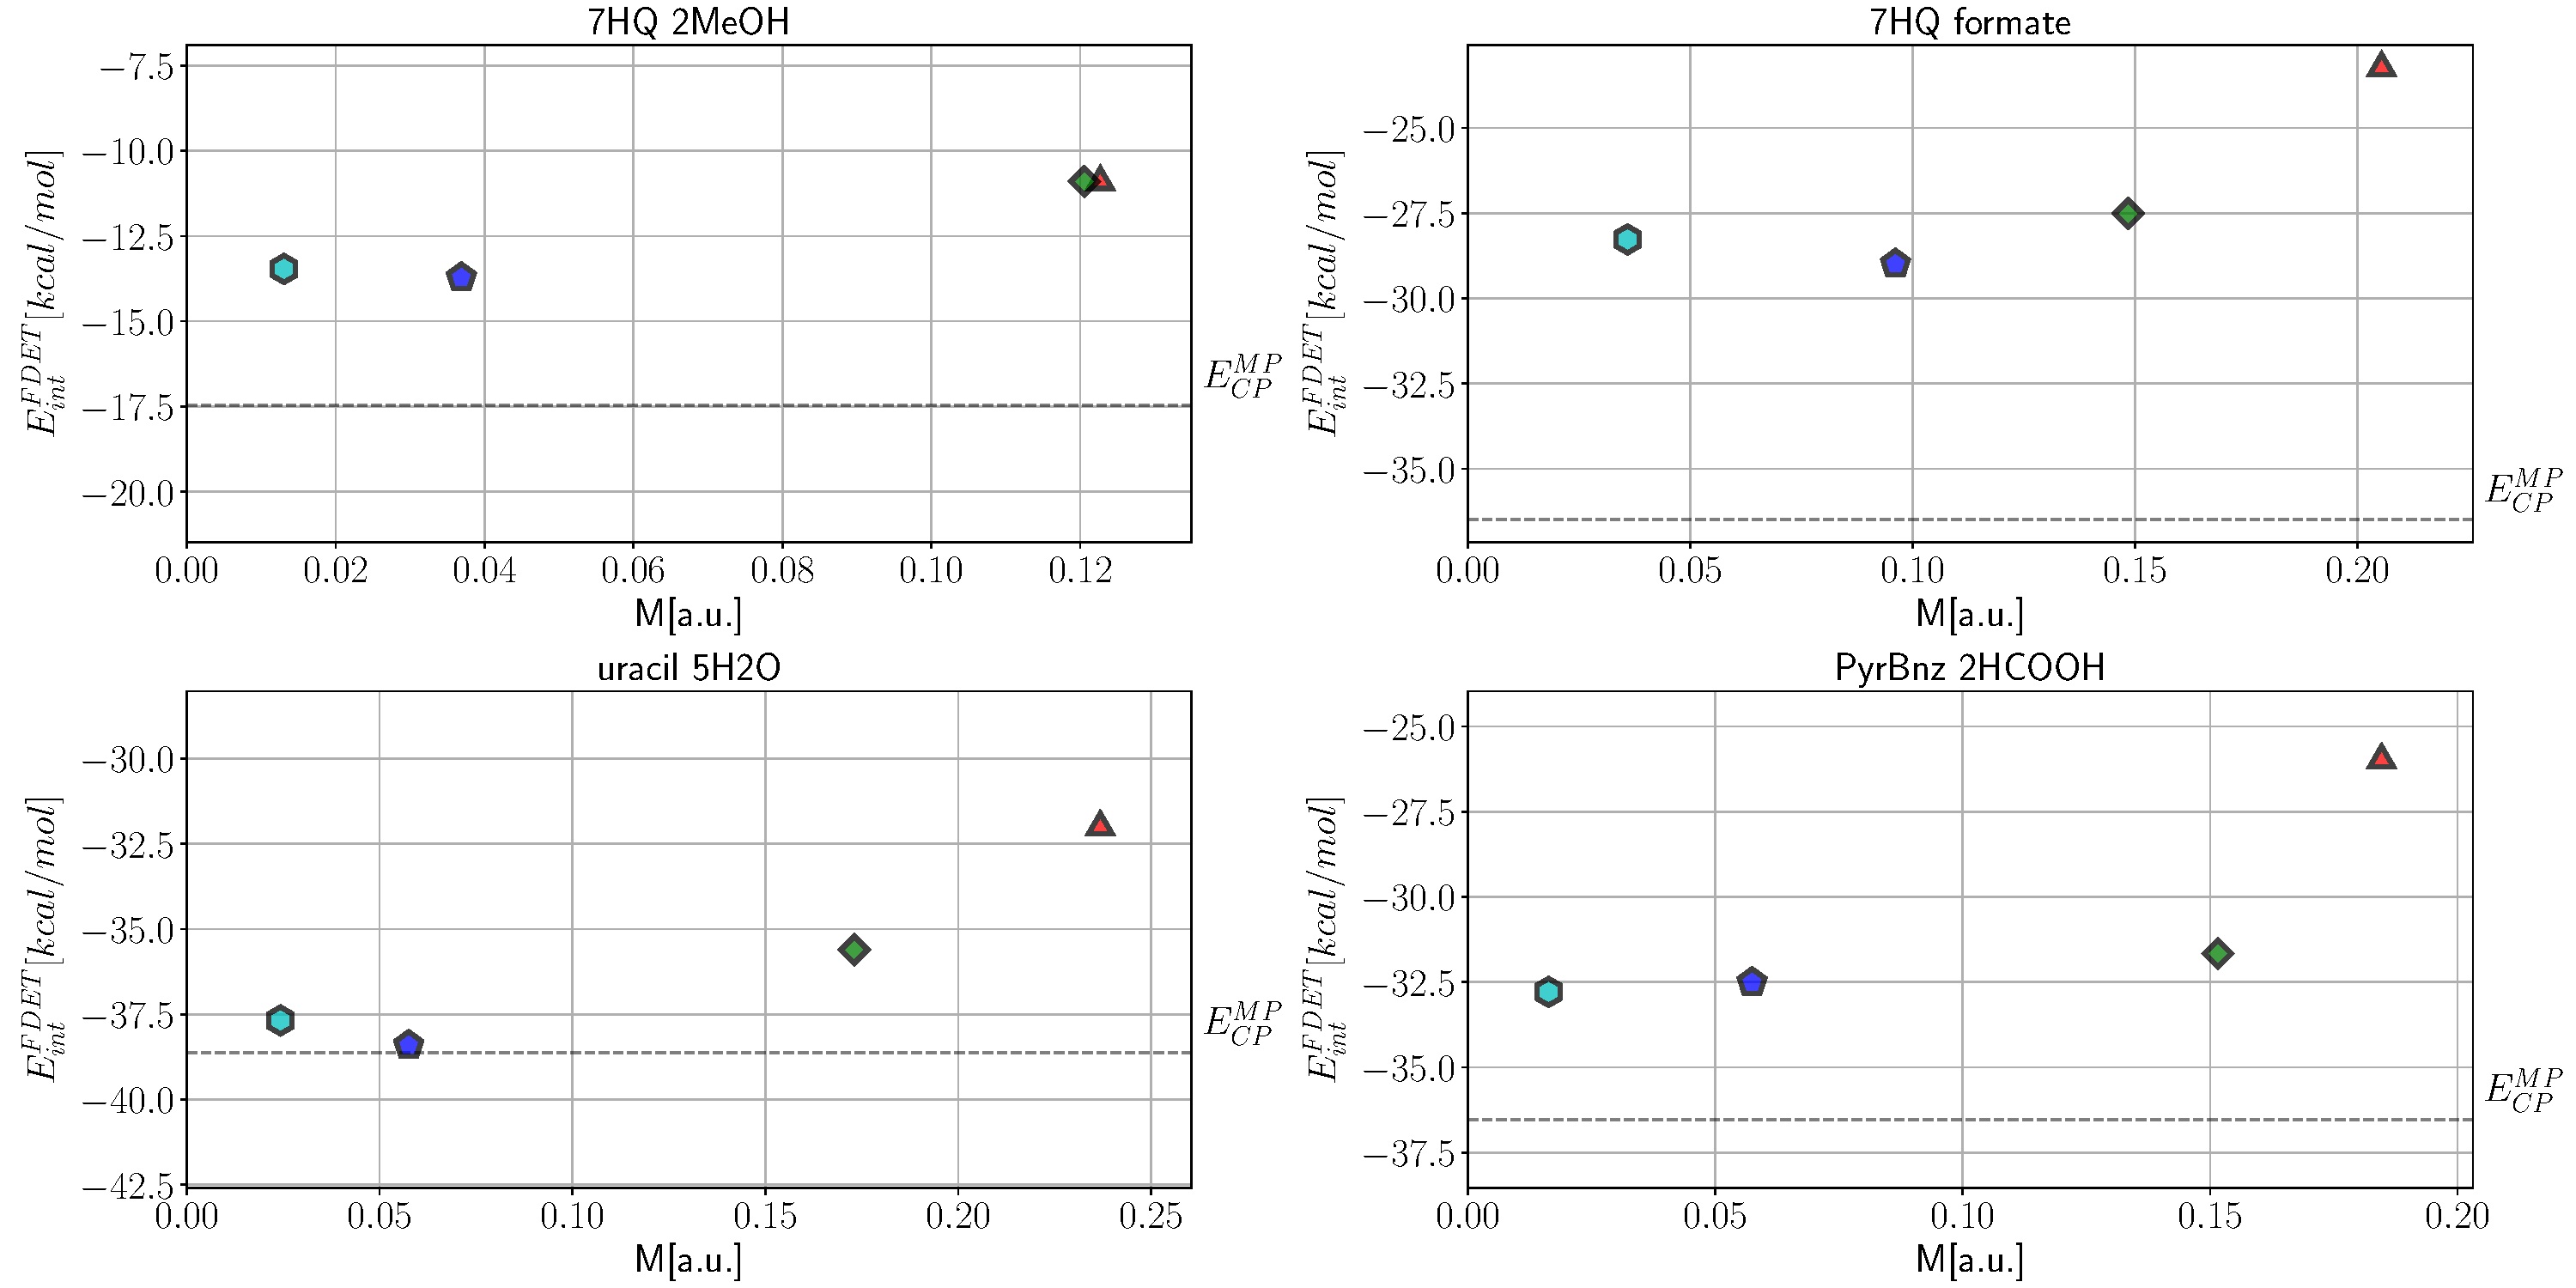
\includegraphics[width=1.0\linewidth]{M_vs_MP.pdf}
\caption{Integrated negative density $M$ and the FDET-MP2 interaction energy for various choices of $\rho_B$: a) $\rho_B^{isol}$ (orange triangles), b) $\rho_B^{FAT}$ (light blue hexagons), c) $\rho_B^{pp(Mulliken)}$ (green diamonds), and d) $\rho_B^{pp(ChelPG)}$ (dark blue pentagons). Data obtained using the {\it monomer expansion}. Horizontal lies indicate the reference interaction energy.}
\label{fig:M_vs_MP}
\end{figure*}

Figure \ref{fig:M_vs_P} shows that the pre-polarisation of $\rho_B$ using the ChelPG representation of $\rho_A^{isol}$
results also in a significant improvement in the total density.
\begin{figure*}
\centering
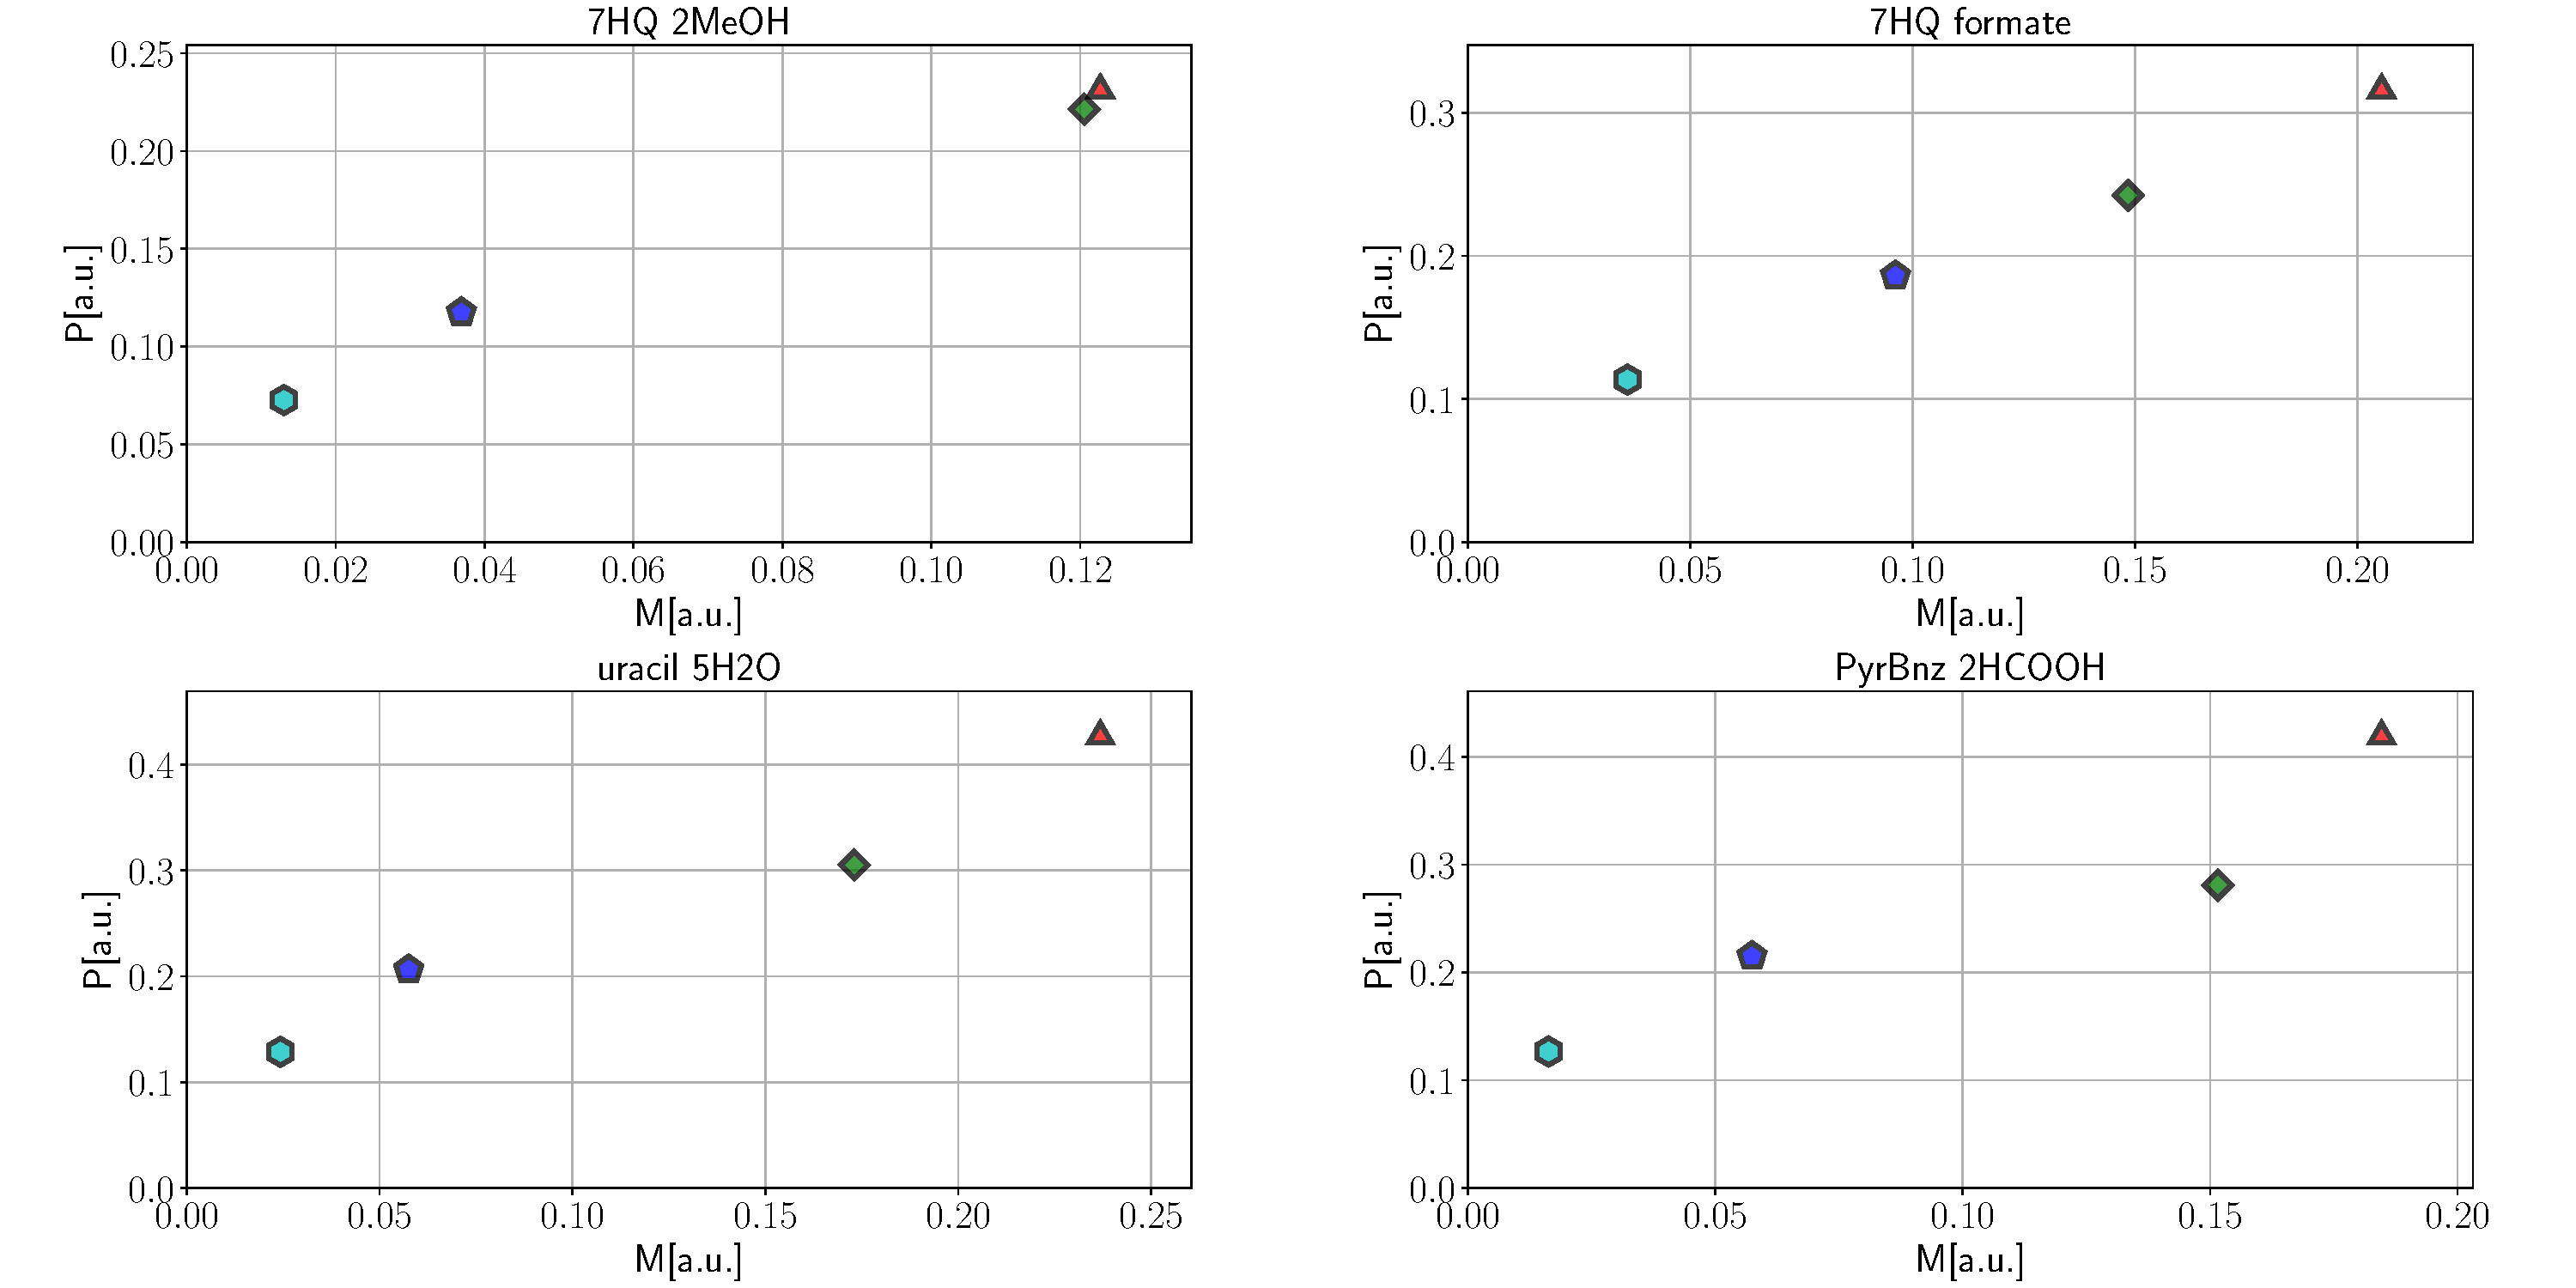
\includegraphics[width=1.0\linewidth]{M_vs_P.pdf}
\caption{Integrated negative density $M$ and the total density error $P$ for various choices of $\rho_B$: a) $\rho_B^{isol}$ (orange triangles), b) $\rho_B^{FAT}$ (light blue hexagons), c) $\rho_B^{pp(Mulliken)}$ (green diamonds), and d) $\rho_B^{pp(ChelPG)}$ (dark blue pentagons). Data obtained using the {\it monomer expansion}.}
\label{fig:M_vs_P}
\end{figure*}
\section{Conclusions}
The present work shows comprehensively that the error in the energy and the density due to the used semi-local approximations for 
${E}_{xcT}^{nad}[\rho_A,\rho_B]$ is significantly smaller than the error in these quantities due to the use of the density of the isolated environment as $\rho_B$ in FDET.
This fact lies at the origin of a remarkable performance of such FDET-based calculations if such density is used \cite{Ricardi2018}.
Whereas the approximation to ${E}_{xcT}^{nad}[\rho_A,\rho_B]$ can result in positive or negative energy error for a given electronic state, the energy error due to such a choice of $\rho_B$ is always non-negative (cf. Eq.~\ref{eq:nfund}). The origin of the good description of vertical excitation energies lies, therefore, in a systematic cancellation of these non-negative contributions for each state.

For the energy of one state, on the other hand, there is no other component that could compensate the error due to violation of this condition. In practical calculations, verification of the condition of the non-negativity of $\rho^{o}_{AB}-\rho_B$ is not possible. This would require \textit{a priori} knowledge of the total density.
The present work provided a link between the violation of the condition of the non-negativity of $\rho^{o}_{AB}-\rho_B$
and the effect of electronic polarisation of $\rho_B$ by the embedded species. Due to this link, the magnitude
of the violation of the non-negativity condition of $\rho^{o}_{AB}-\rho_B$ can be significantly reduced in practice.
\section*{Supplementary Material}
The Supplementary material includes the proof of Eq.~\ref{eq:P_bound}, the magnitude of the counterpoise corrections for $E_{int}^{ref}$, and the values of $E_k[\Delta \rho^{c}_{v'_X}, \rho'_X, \rho_Y]$ for the different calculations.
Any additional data is made available on request from the authors.
\bibliography{biblio}

\end{document}
